% !TeX root = ../main.tex

\chapter{Reproducibility Information}\label{appendix:reproducibility}

\section{Experiment Inventory}
\label{app:results-repository}

The repository accompanying this thesis provides the experimental results
and the web-based experiment management and visualization tool introduced
in \autoref{sec:contributions}. The tool supports experiment configuration,
job-script generation, run management, and visualization of measured
results. The repository is available at:
\begin{quote}
\url{https://github.com/jintaolutum-dev/mpi-async-overlap-stud}
\end{quote}

% TODO: Map each figure and table to raw runs and analysis scripts.

\section{Message-Size Overlap Figure Set}\label{app:message-size-overlap-figures}

The following figures compare asynchronous progress disabled (Case~01)
and enabled (Case~03) across the complete message-size sweep for each
MPI implementation and transport configuration. All figures use the
\texttt{cm4\_inter} two-node, two-rank configuration and the MPI
\texttt{seq/seq-seq} policy. Each curve shows the mean measured overlap
across the experimental runs.

\begin{figure}[p]
    \centering
    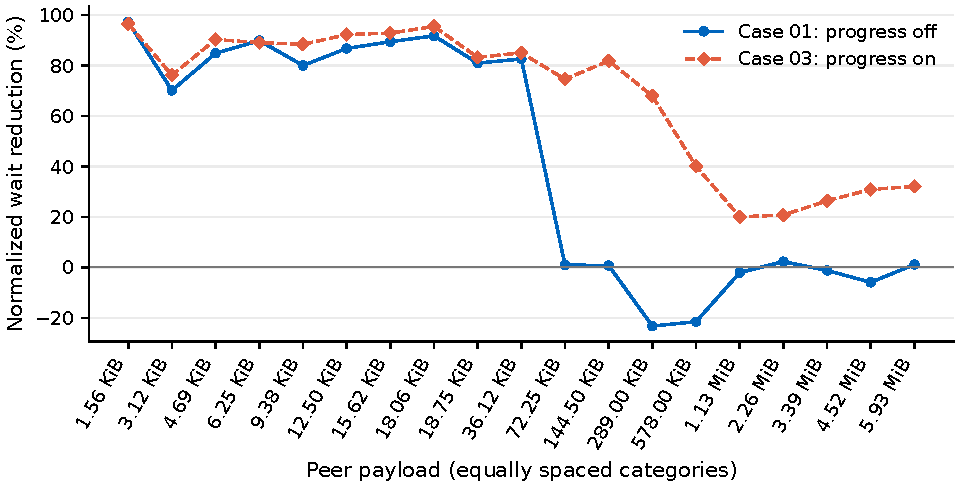
\includegraphics[width=\textwidth]{figures/on_off/inter-openmpi-case01-06-overlap-vs-message-size.pdf}
    \caption[Open MPI TCP asynchronous progress off versus on.]{Open MPI TCP: measured overlap across 19 peer payloads with
        asynchronous progress disabled (Case~01, solid line with circles,
        24 application threads) and enabled (Case~03, dashed line with diamonds,
        23 application threads and one CPU reserved for progress).
        Both cases use \texttt{wait\_all} and \texttt{seq/seq-seq} in the
        two-node, two-rank \texttt{cm4\_inter} configuration.}
    \label{fig:app-openmpi-progress-on-off}
\end{figure}

\begin{figure}[p]
    \centering
    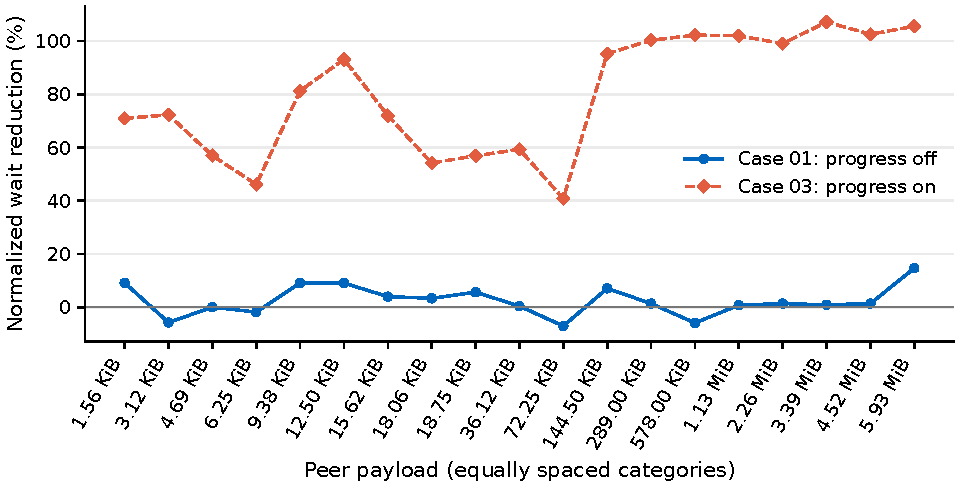
\includegraphics[width=\textwidth]{figures/on_off/inter-intelmpi-case01-06-overlap-vs-message-size.pdf}
    \caption[Intel MPI verbs asynchronous progress off versus on.]{Intel MPI verbs: measured overlap across 19 peer payloads with
        asynchronous progress disabled (Case~01, solid line with circles,
        24 application threads) and enabled (Case~03, dashed line with diamonds,
        23 application threads and one CPU reserved for progress).
        Both cases use \texttt{wait\_all} and \texttt{seq/seq-seq} in the
        two-node, two-rank \texttt{cm4\_inter} configuration.}
    \label{fig:app-intelmpi-verbs-progress-on-off}
\end{figure}

\begin{figure}[p]
    \centering
    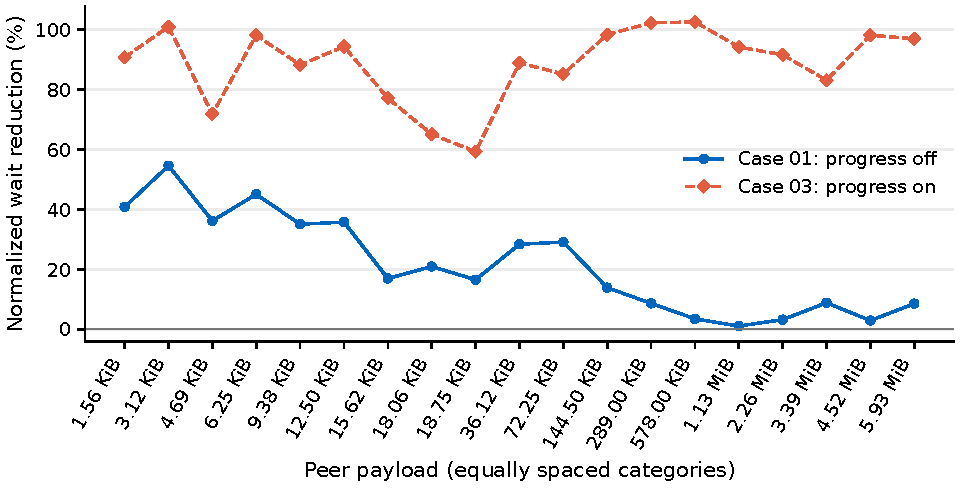
\includegraphics[width=\textwidth]{figures/on_off/inter-intelmpi_tcp-case01-06-overlap-vs-message-size.pdf}
    \caption[Intel MPI TCP asynchronous progress off versus on.]{Intel MPI TCP: measured overlap across 19 peer payloads with
        asynchronous progress disabled (Case~01, solid line with circles,
        24 application threads) and enabled (Case~03, dashed line with diamonds,
        23 application threads and one CPU reserved for progress).
        Both cases use \texttt{wait\_all} and \texttt{seq/seq-seq} in the
        two-node, two-rank \texttt{cm4\_inter} configuration.}
    \label{fig:app-intelmpi-tcp-progress-on-off}
\end{figure}

\begin{figure}[p]
    \centering
    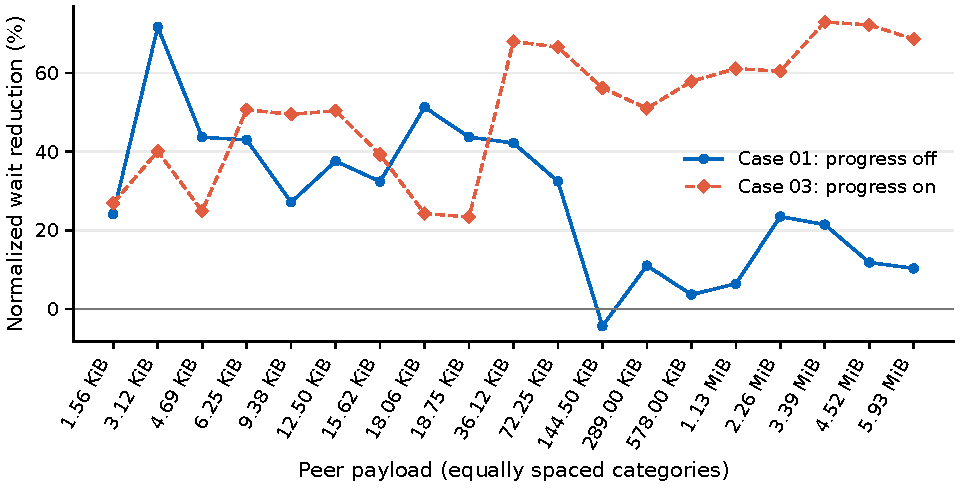
\includegraphics[width=\textwidth]{figures/on_off/inter-mpich-case01-06-overlap-vs-message-size.pdf}
    \caption[MPICH TCP asynchronous progress off versus on.]{MPICH TCP: measured overlap across 19 peer payloads with
        asynchronous progress disabled (Case~01, solid line with circles,
        24 application threads) and enabled (Case~03, dashed line with diamonds,
        23 application threads and one CPU reserved for progress).
        Both cases use \texttt{wait\_all} and \texttt{seq/seq-seq} in the
        two-node, two-rank \texttt{cm4\_inter} configuration.}
    \label{fig:app-mpich-progress-on-off}
\end{figure}


